\chapter{Wyznaczanie średnicy}
Problem średnicy dowolnego zbioru punktów można przedstawić
następująco: jeśli danych jest $N$ punktów na płaszczyźnie, znaleźć
dwa punkty najbardziej odległe od siebie. Problem można rozwiązać
metodą naiwną wyznaczając odległość wszystkich $N(N-1)/2$ par punktów
i wybierając największą z nich. Naturalnym jest jednak szukanie
bardziej efektywnych rozwiązań.

Aby uniknąc badania wszystkich par punktów, można skoorzystać z
twierdzenia \ref{thm:hy61}, wyznaczając otoczkę wypukłą zbioru
punktów w czasie oczekiwanym $O(n \log n)$, a następnie wyznaczając
jej średnicę.

\begin{twierdzenie}[Hocking-Young 1961\label{thm:hy61}]

  Średnica zbioru jest równa średnicy jego otoczki wypukłej.
\end{twierdzenie}

Wiemy, że zbiór wierzchołków wielokąta wypukłego jest jego otoczką
wypukłą, dlatego zdefiniujmy następujący problem:

\begin{problem}[Średnica wielokąta wypukłego]
  Jeśli dany jest wielokąt wypukły, znaleźć jego średnicę,
  tj.\ największą odległość pomiędzy dowolną parą jego wierzchołków.
\end{problem}

% Wiemy, że istnieje algorytm o złożoności $O(n\log{n})$,
% przekształcając problem rozłączności zbiorów w problem średnicy [1].
% Warto więc zastanowić się czy właściwości wielokąta wypukłego pomogłby
% nam uzyskać lepszy algorytm dla uzyskania średnicy zbioru. Skorzystamy
% z następującego twiedzenia:

% % nawiązać do spostrzeżenia, że problem 'średnica zbioru' zawiera się
% % w/lub równa 'srednica wielokąta wypukłego'

Kluczowym dla algorytmu korzystającego z wypukłości wielokąta przy
wyznaczaniu średnicy jest następujące twierdzenie:

\begin{twierdzenie}[Yaglom-Bolyanskii 1961]
\label{thm:yagbol}
  Średnica figury wypukłej jest największa odległością między parą
  równoległych prostych wspierających.
\end{twierdzenie}

% idea algorytmu
Proste wspierające nie mogą przechodzić przez każdą parę punktów. Na
przykład żadne proste wpierające przechodzące przez $p_1$ i $p_5$
wielokąta z rysunku \ref{fig:antipodal} nie mogą być równoległe, więc
$p_{1}p_{5}$ nie jest średnicą. Para punktów, przez które mogą
przechodzić proste wspierające, jest nazywana punktami
\emph{antypodycznymi}. Z twierdzenia \ref{thm:yagbol} wynika, że
szukając średnicy nie musimy badać wszystkich par punktów, a jedynie
pary antypodyczne.

\begin{figure}[htp]
\centering
  \begin{tikzpicture}[scale=0.8]
    \convexA

      \node [anchor=center,circle,draw,fill,inner sep=0.5pt,
      label={right:$p_0$}] at (p0) {};

      \node [anchor=center,circle,draw,fill,inner sep=0.5pt,
      label={45:$p_1$}] at (p1) {};

      \node [anchor=center,circle,draw,fill,inner
      sep=0.5pt,label={above:$p_2$}] at (p2) {};

      \node [anchor=center,circle,draw,fill,inner
      sep=0.5pt,label={135:$p_3$}] at (p3) {};

      \node [anchor=center,circle,draw,fill,inner
      sep=0.5pt,label={left:$p_4$}] at (p4) {};

      \node [anchor=center,circle,draw,fill,inner
      sep=0.5pt,label={below:$p_5$}] at (p5) {};

      \node [anchor=center,circle,draw,fill,inner
      sep=0.5pt,label={315:$p_6$}] at (p6) {};

  \end{tikzpicture}
\caption{\label{fig:antipodal}}
\end{figure}

Przedstawiony zostanie teraz sposób znajdowania par punktów
antypodycznych. Rozważmy wielokąt przedstawiony na
rysunku \ref{fig:antipodal}. Wybieramy dowolny wierzchołek $p_i$ i
przechodzimy w kierunku przeciwnym do ruchu wskazówek zegara po brzegu
wielokąta tak długo, aż dojdziemy do wierzchołka $q_r$, który jest
najdalej od prostej zawierającej krawędź $p_{i}p_{i-1}$. W taki sam
sposób wyznaczamy wierzchołek $q_l$ jako najdalszy od $p_{i}p_{i+1}$
przechodząc po brzegu wielokąta zgodnie z ruchem wskazówek
zegara. Łańcuch $C(p_i)$ wierzchołków od $q_r$ do $q_l$, z nimi samymi
włącznie, przeciwnie do ruchu wskazówek zegara, tworzy zbiór
wierzchołków, z których każdy tworzy parę antypodyczną z $p_i$. Możemy
zauważyć, że ($p_{i},p_{r}$) jest parą antypodyczną wyłącznie wtedy,
gdy istnieje prosta przecinająca $\angle \alpha_i$ i $\angle \alpha_s$
(rys. \ref{fig:diameter}). Ze względu na to, że $C(p_i)$ jest
łańcuchem wypukłym, każdy wierzchołek $p_s$ należący do $C(p_i)$ jest
antypodyczny do $p_i$, a żaden wierzchołek nienależący do $C(p_i)$
takim nie jest. Fakt ten umożliwia konstrukcję algorytmu pozwalającego
efektywnie uzyskać wszystkie pary antypodyczne.

\begin{figure}[htp]
  \centering
  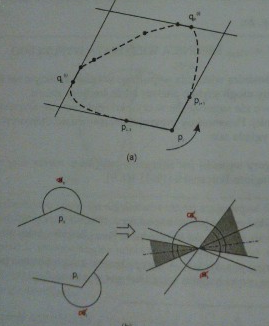
\includegraphics[width=0.3\textwidth]{img/diameter}
  \caption{[Rysunek roboczy]\label{fig:diameter}}
\end{figure}

% działanie algorytmu
Wejściem dla algorytmu jest wielokąt zadany jako lista wierzchołków ze
wskaźnikiem na swój następnik. Do określenia, który punkt leży
najdalej od odcinka $p_{0}p_{i+1}$ korzystamy funkcji ,,pola ze
znakiem trójkąta'' $p_{0}p_{i+1}p$, którą przedstawiono w
rozdziale \ref{chap:pojecia} do wyznaczenia skrętności kąta, w
algorytmie oznaczonej jako $P$. W pierwszej części algorytmu w pętli
\texttt{while} szukamy pierszego najdalszego wierzchołka i oznaczamy
go jako $q_0$ (wiersze 4--6). Następnie wyznaczamy łańcuch $C(p_i)$,
używając wskaźników $p$ i $q$ poruszających się w kierunku odwrotnym
do ruchu wskazówek zegara zaczynając odpowiednio od $p_0$ i $q_0$ do
momentu, aż wskaźnik $q$ wróci do pozycji $p_0$ (wiersze 7--14). Po
tym kroku zostaną wypisane wszystkie pary antypodyczne. Znalezienie
wierzchołka $q_0$ zajmuje w pesymistycznym przypadku $N-1$ kroków,
natomiast przejście po łańuchach $p_{0}q_{0}$ i $q_{0}p_{0}$ łącznie
$N$ kroków. Specjalną sytuacją jest przypadek, gdy dwie krawędzie są
równoległe (wtedy pole ze znakiem trójkąta jest równe dla dwóch
wierzchołków tworzących krawędź równoległą), która wymaga od nas
dodatkowego kroku przy każdym wierzchołku (wiersze 15--19).

Poprawność algorytmu wynika z tego, że krawędzi równoległych jest co
najwyżej $N/2$, więc łącznie algorytm nie wykonuje więcej niż $3N$
kroków. Mamy więc do czynienia ze złożonością czasową rzędu $O(n)$.

% poprawność
Punkt antypodyczny dla punktu $p_{i+1}$ nie może być on bliższy niż
wierzchołek, który jest najdalej od $p_i$. Związane jest to z
wypukłością wielokąta --- dla dowolnego wierzchołka $p$ można
wyznaczyć taki wierchołek $q$, że odległość kolejnych wierzchołków od
$p$ do $q$ jest nierosnąca, zaś od $q$ do $p$ niemalejąca.

\begin{figure}[htp]

\begin{algorithmic}[1]
\Procedure{Antipodal Pairs}{}

\State $p \gets p_N$
\State $q \gets NEXT[p]$

\While {$P(p, NEXT[p], NEXT[q]) > P(p,NEXT[p],q)$}
    \State $q \gets NEXT[p]$
    \State $q_0 \gets q$

    \While {$q \neq p_0$}
        \State $print (p, q)$

        \While {$P(p, NEXT[p], NEXT[q] > P(p, NEXT[p], q))$}
            \State $q \gets NEXT[q]$

            \If {$(p, q) \neq (q_0,p_0)$}
                \State $print (p, q)$
            \EndIf
        \EndWhile

        \If {$P(p, NEXT[p], NEXT[q] = P(p, NEXT[p], q))$}
            \If {$(p, q) \neq (q_0, p_n)$}
                \State $print (p, NEXT[q])$
            \EndIf
        \EndIf
    \EndWhile
\EndWhile
\EndProcedure

\end{algorithmic}
\caption{\label{alg:antipodal}}
\end{figure}

%%% Local Variables:
%%% mode: latex
%%% TeX-master: "masterthesis"
%%% TeX-engine: xetex
%%% End:
